\section{Expected Results: Experimental results, deliverables, demos etc.}

In this section, we describe the results of the performed evaluation.

\subsection{Preliminary results}

In the early stages of the development of the described architecture
(see Section~\ref{sec:Approach}), we have performed a preliminary
configuration of the targeted board to: 1) boot the two embedded
cores; 2) program the FPGA to allow a basic interconnection between
embedded processor and GPIOs; 3) instantiate a timer device; 4) test
the functionaloty of GPIO, timer and UART interface.

\begin{figure*}[t]
  \centering
  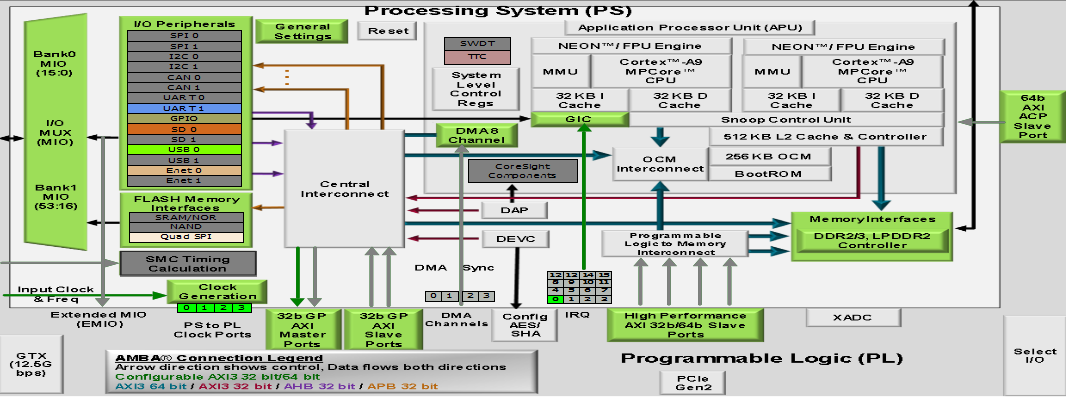
\includegraphics[width=1\textwidth]{fig/proc_bare.png}
  \caption{Instantiation of the embedded processor with basic
    interconnection logic between I/O peripherals and processor
    subsystem.}
  \label{fig:proc}
\end{figure*}

Figure~\ref{fig:proc} shows an overview of the preliminary
configuration of the board through the Xilinx Platform Studio. As can
be seen, the ARM CPUs have been instantiated together with a central
interconnect. Moreover, a timer peripheral has been routed to the
Generic Interrupt Controller (GIC).

As previously mentioned, a bare-metal application has been deployed,
which performs the following operations:

\begin{enumerate}
\item Initialize GPIO devices
\item Initialize UART interface
\item Wait for GPIO input through push-buttons
\item Setup a timer interrupt
\item Performs GPIO output upon arrival of the timer interrupt
\item Provides a feedback of the operation being performed thorugh
  UART
\end{enumerate}

\subsection{Expected results}

In the next steps, we plan to perform the porting of a simple OS that
allows the definition of a complete task-set with parameters and that
performs the export of said parameters to a memory locations that are
shared beteween the embedded processor and the FPGA. In this way, we
will be able to implement and test a basic communication interface
between the application layer and the programmable block.

As a further step, we will implement a basic scheduler on the FPGA
module that will represent the LST hardware scheduler after
successive, iterative refinements. We plan to close the loop having
the implemented hardware LST scheduler generating interrupt for the
embedded processor and implementing the context-switch mechanism on
the ARM core as a fast-IRQ handler.

We plan to investigate the achieved performances in terms of CPU
utilization and schedulability that are achievable on the proposed
architecture, as well as understanding the power consumption of the
implemented scheduler.

We expect to observe a significative reduction of the scheduling
overhead in comparison with software-based implementations. Moreover,
we expect to observe an optimal assignment of task to CPUs that will
allow an overall utilization close to the theoretical
maximum. Finally, we expect a reduced FPGA area utilization if
compared to the implementation in~\cite{GUPTA10}, as well as a
reduction in the power consumption.
